\documentclass[11pt,letterpaper]{article}
\usepackage[margin=.68in]{geometry}
\usepackage[T1]{fontenc}
\usepackage{lmodern,microtype,booktabs,array,graphicx,xcolor,amsmath,hyperref}
\hypersetup{colorlinks=true,urlcolor=blue,linkcolor=blue,pdftitle={Return a range when supplier data are incomplete}}
\setlength{\parindent}{0pt}\setlength{\parskip}{6pt}
\newcommand{\heading}[1]{\vspace{4pt}{\large\bfseries #1}\par}
\newcommand{\BoundA}{41}
\newcommand{\BoundB}{456}
\newcommand{\BoundC}{4}
\newcommand{\BoundD}{454,708.41}
\newcommand{\BoundE}{480}
\newcommand{\BoundF}{1,440}
\newcommand{\BoundG}{11,520}
\newcommand{\BoundH}{79.478498}
\newcommand{\BoundI}{179}
\newcommand{\BoundJ}{140}
\newcommand{\BoundK}{39}
\newcommand{\BoundL}{17}
\newcommand{\BoundM}{10,424,423.36}
\newcommand{\BoundN}{10,238,325.51}
\newcommand{\BoundO}{186,097.85}
\newcommand{\BoundP}{98.214790}
\newcommand{\BoundQ}{3,844,805.77}
\newcommand{\BoundR}{3,707,262.33}
\newcommand{\BoundS}{137,543.44}
\newcommand{\BoundT}{96.422617}
\newcommand{\BoundU}{1,848,993.46}
\newcommand{\BoundV}{1,600,096.20}
\newcommand{\BoundW}{248,897.26}
\newcommand{\BoundX}{86.538770}
\newcommand{\BoundY}{8,969,215.42}
\newcommand{\BoundZ}{8,926,870.08}
\newcommand{\BoundAA}{42,345.34}
\newcommand{\BoundAB}{99.527881}
\newcommand{\BoundAC}{5,521,529.24}
\newcommand{\BoundAD}{4,388,428.50}
\newcommand{\BoundAE}{1,133,100.74}
\newcommand{\BoundAF}{79.478498}
\newcommand{\BoundAG}{2,237,133.82}
\newcommand{\BoundAH}{1,924,502.76}
\newcommand{\BoundAI}{312,631.06}
\newcommand{\BoundAJ}{86.025375}
\newcommand{\BoundAK}{72}
\newcommand{\BoundAL}{48}
\newcommand{\BoundAM}{0}
\newcommand{\BoundAN}{0}
\newcommand{\BoundAO}{72}
\newcommand{\BoundAP}{36}
\newcommand{\BoundAQ}{12}
\newcommand{\BoundAR}{0}
\newcommand{\BoundAS}{72}
\newcommand{\BoundAT}{36}
\newcommand{\BoundAU}{12}
\newcommand{\BoundAV}{0}
\newcommand{\BoundAW}{69}
\newcommand{\BoundAX}{51}
\newcommand{\BoundAY}{0}
\newcommand{\BoundAZ}{0}
\newcommand{\BoundBA}{69}
\newcommand{\BoundBB}{37}
\newcommand{\BoundBC}{14}
\newcommand{\BoundBD}{0}
\newcommand{\BoundBE}{69}
\newcommand{\BoundBF}{34}
\newcommand{\BoundBG}{17}
\newcommand{\BoundBH}{0}
\newcommand{\BoundBI}{65}
\newcommand{\BoundBJ}{43}
\newcommand{\BoundBK}{0}
\newcommand{\BoundBL}{12}
\newcommand{\BoundBM}{65}
\newcommand{\BoundBN}{40}
\newcommand{\BoundBO}{3}
\newcommand{\BoundBP}{12}
\newcommand{\BoundBQ}{65}
\newcommand{\BoundBR}{37}
\newcommand{\BoundBS}{6}
\newcommand{\BoundBT}{12}
\newcommand{\BoundBU}{63}
\newcommand{\BoundBV}{45}
\newcommand{\BoundBW}{0}
\newcommand{\BoundBX}{12}
\newcommand{\BoundBY}{63}
\newcommand{\BoundBZ}{42}
\newcommand{\BoundCA}{3}
\newcommand{\BoundCB}{12}
\newcommand{\BoundCC}{63}
\newcommand{\BoundCD}{39}
\newcommand{\BoundCE}{6}
\newcommand{\BoundCF}{12}
\newcommand{\BoundCG}{41}
\newcommand{\BoundCH}{456}
\newcommand{\BoundCI}{2020}
\newcommand{\BoundCJ}{Canada}
\newcommand{\BoundCK}{0}
\newcommand{\BoundCL}{0.5}
\newcommand{\BoundCM}{1,488,313.00}
\newcommand{\BoundCN}{0.00}
\newcommand{\BoundCO}{1,446,978.26}
\newcommand{\BoundCP}{41,334.74}
\newcommand{\BoundCQ}{1,488,313.00}
\newcommand{\BoundCR}{0}
\newcommand{\BoundCS}{0.00}
\newcommand{\BoundCT}{3}
\newcommand{\BoundCU}{454,708.41}
\newcommand{\BoundCV}{0}
\newcommand{\BoundCW}{0.00}
\newcommand{\BoundCX}{1}
\newcommand{\BoundCY}{53,231.15}
\newcommand{\BoundCZ}{179}
\newcommand{\BoundDA}{145,694}
\newcommand{\BoundDB}{145,694}
\newcommand{\BoundDC}{37}
\begin{document}
{\LARGE\bfseries Return a range when supplier data are incomplete\par}
\vspace{5pt}Independent research program\hfill 31 October 2026 UTC\\
\textit{Not peer reviewed. Source-informed 2019/2020 wheat-network scenario arithmetic.}

\heading{Practical finding}
A planner should not turn missing supplier information into a single replacement promise. Under the full authored outside-capacity envelope, \BoundA{} of \BoundB{} positive-loss configurations cannot determine full replacement from the known network alone. The upper endpoint can cover modeled demand; the known-only endpoint cannot. Those cases require supplier-specific availability evidence before a delivery commitment.

Separate-country calculations also overclaim a shared supplier pool in \BoundC{} known-only configurations, all on the exporter-mirror basis, with a maximum gap of \BoundD{} tonnes. No import-basis configuration in this grid has a positive shared-capacity gap. The comparison retains this negative finding rather than implying that every replacement calculation double counts supply.

\heading{What the product returns}
The implementation returns a conditional interval for optimal covered and unmet mass under an explicit historical scenario and outside-capacity contract. It returns an unresolved classification when outside availability determines whether full modeled replacement is possible. It does not promise cargo, estimate a current shortage probability or allocate political priority.

The exercise retains all \BoundE{} base configurations, \BoundF{} endpoint evaluations and \BoundG{} exact cut-subset certificates. Both years, both source bases, every loss origin and every parameter setting remain available underneath the first-layer finding.

\heading{An earlier failed question is preserved}
The original coverage-gated network study remains unexecuted. Morocco's 2020 FAO common-import share is \BoundH{}\%, below its unchanged 80\% gate. The original UN attempt also remains failed. This distinct source-informed exercise models a restricted known network and explicit outside-capacity uncertainty; it does not pass, relax or rename that original source requirement.

\heading{The important limitation}
The accounting residual is not measured spare supply. All additional shared supply, route multipliers and outside caps are authored assumptions, applied to compiled historical records. The results are exact within those constraints, with no physical-delivery, food-security, causal, predictive, adoption, scientific-priority or realized-savings claim.

\newpage
\heading{Source support and the signed accounting residual}
Use only the separately captured FAO/FAOSTAT projection: Egypt, Morocco and Tunisia; ten fixed origins; Wheat grain item 15/CPC0111; TM bilateral import/export quantities and TCL national totals. Tonnes are converted exactly to kg without increasing measurement precision. The public projection preserves \BoundI{} requested source positions: \BoundJ{} positive and \BoundK{} missing. Among positive positions, \BoundL{} carry flag I (imputed by a receiving agency); other positive positions carry A (official value). These positions are not independent shipment observations.

A current modeled edge requires positive import and exporter-mirror quantities. Both bases use the identical common-support intersection, while retaining their differing amounts. The signed residual is national imports minus the common-support import-reported mass. All six are nonnegative; no discrepancy is clamped. This residual can reflect omitted flows, source revisions or accounting differences. It is a scale for an authored sensitivity envelope, not a fact-derived future-supply cap.

\begin{center}\small\begin{tabular}{llrrrr}\toprule
Importer & Year & National (t) & Common (t) & Residual (t) & Share (\%)\\\midrule
Egypt & 2019 & \BoundM{} & \BoundN{} & \BoundO{} & \BoundP{}\\
Morocco & 2019 & \BoundQ{} & \BoundR{} & \BoundS{} & \BoundT{}\\
Tunisia & 2019 & \BoundU{} & \BoundV{} & \BoundW{} & \BoundX{}\\
Egypt & 2020 & \BoundY{} & \BoundZ{} & \BoundAA{} & \BoundAB{}\\
Morocco & 2020 & \BoundAC{} & \BoundAD{} & \BoundAE{} & \BoundAF{}\\
Tunisia & 2020 & \BoundAG{} & \BoundAH{} & \BoundAI{} & \BoundAJ{}\\
\bottomrule\end{tabular}\end{center}
\begin{center}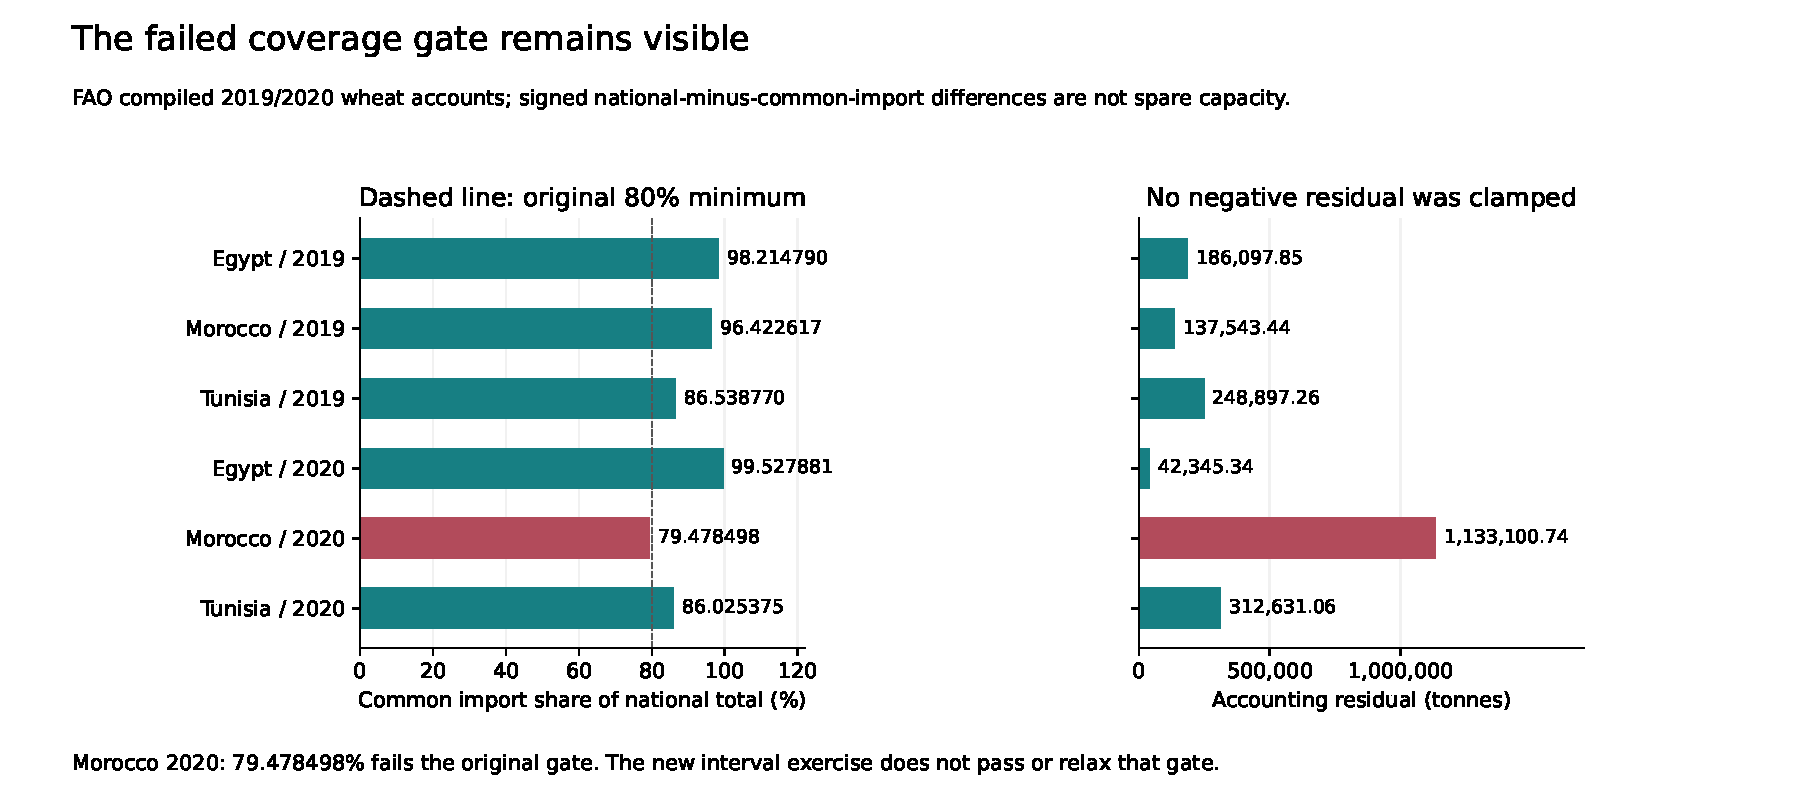
\includegraphics[width=\linewidth]{images/coverage_and_residual.pdf}\end{center}
The source is compiled and later revised: observed TM/TCL update dates differ, in December 2025 and July 2026. Current historical captures do not recover original operational delivery vintages. Preserve the source-specific country definitions and reporting limitations in FAO\_SOURCE\_PLAN.md. Import and mirror agreement is not independent ground truth. No UN quantity is mixed into these calculations.

\newpage
\heading{Known-network model and authored parameter grid}
For target year $y$ and lost origin $k$, replacement demand $d_i$ is its qualified current-basis amount to importer $i$. Other origin $j$ has hypothetical extra shared supply $s_j=\alpha X_{j,y-1}$ from prior national exports. Its extra route cap is $c_{ji}=\beta M_{ji,y-1}$ on a positive observed prior import link. Lost origin $k$ supplies no replacement. An unavailable route is excluded from this restricted model, not proven physically impossible.

Maximize total covered kg with nonnegative route flows $x_{ji}$ subject to
\[
 \sum_i x_{ji}\le s_j,\qquad x_{ji}\le c_{ji},\qquad
 \sum_j x_{ji}\le d_i.
\]
Use $\alpha\in\{0,.05,.10,.25\}$ and $\beta\in\{.5,1,2\}$, ten complete-origin losses, two current bases and both years. Nothing is fitted or selected. The objective maximizes total modeled coverage; tied allocations do not optimize fairness, nutrition, price or national welfare. Numeric code order makes the returned allocation deterministic.

\heading{Conditional uncertainty class and sharp endpoint bounds}
Let $r_i=W_i-C_i\ge0$ be the accounting residual and $\gamma\in\{0,1/2,1\}$. A virtual outside origin has unknown shared capacity $b$ and route capacities $u_i$ in the class
\[
 0\le b\le\gamma\sum_i r_i,\qquad 0\le u_i\le\gamma r_i.
\]
This is an authored outside-supply model; it is not implied by past imports. Let $F_0$ be the known-only optimum and $F_\gamma$ the optimum at all upper outside capacities. Capacity monotonicity gives $F_0\le F(b,u)\le F_\gamma$. Zero outside capacities attain the lower endpoint and all upper capacities attain the upper endpoint. Thus these are sharp conditional bounds. Unmet mass lies in $[D-F_\gamma,D-F_0]$, where $D=\sum_i d_i$.

Without a finite outside-capacity assumption, the same known-network assumptions allow the wider interval $[F_0,D]$: sufficiently large added routes can cover all modeled demand. Never substitute the residual-capped upper value for a data-identified real-world upper bound.

\heading{Independent finite optimality certificate}
For each of the eight importer-side cut subsets $S$, an origin's best cut placement is independent once $S$ is fixed. The objective is certified by
\[
 F=\min_{S\subseteq I}\left[\sum_{i\in S}d_i+
 \sum_j\min\left(s_j,\sum_{i\notin S}c_{ji}\right)\right].
\]
The virtual origin is included. Every stored nonnegative allocation respects source, route and demand caps and node conservation; its total equals this independently enumerated minimum. This is established max-flow/min-cut reasoning [3], not a new algorithm or a physical feasibility certificate. Separate-country optima each reuse the shared pool, so their sum can exceed the jointly feasible value.

\newpage
\heading{All classification counts, including zero modeled loss}
Each row contains 120 base configurations. K means the known network alone covers modeled demand; S means a shortfall persists even at the conditional upper envelope; U means full replacement depends on unavailable outside-capacity information; Z means zero loss within the restricted modeled support. Z is not proof of zero physical exposure. Loss-normalized ratios are undefined for Z.

\begin{center}\small\begin{tabular}{llrrrrr}\toprule
Year & Basis & $\gamma$ & K & S & U & Z\\\midrule
2019 & import & 0 & \BoundAK{} & \BoundAL{} & \BoundAM{} & \BoundAN{}\\
2019 & import & 1/2 & \BoundAO{} & \BoundAP{} & \BoundAQ{} & \BoundAR{}\\
2019 & import & 1 & \BoundAS{} & \BoundAT{} & \BoundAU{} & \BoundAV{}\\
2019 & mirror & 0 & \BoundAW{} & \BoundAX{} & \BoundAY{} & \BoundAZ{}\\
2019 & mirror & 1/2 & \BoundBA{} & \BoundBB{} & \BoundBC{} & \BoundBD{}\\
2019 & mirror & 1 & \BoundBE{} & \BoundBF{} & \BoundBG{} & \BoundBH{}\\
2020 & import & 0 & \BoundBI{} & \BoundBJ{} & \BoundBK{} & \BoundBL{}\\
2020 & import & 1/2 & \BoundBM{} & \BoundBN{} & \BoundBO{} & \BoundBP{}\\
2020 & import & 1 & \BoundBQ{} & \BoundBR{} & \BoundBS{} & \BoundBT{}\\
2020 & mirror & 0 & \BoundBU{} & \BoundBV{} & \BoundBW{} & \BoundBX{}\\
2020 & mirror & 1/2 & \BoundBY{} & \BoundBZ{} & \BoundCA{} & \BoundCB{}\\
2020 & mirror & 1 & \BoundCC{} & \BoundCD{} & \BoundCE{} & \BoundCF{}\\
\bottomrule\end{tabular}\end{center}
\begin{center}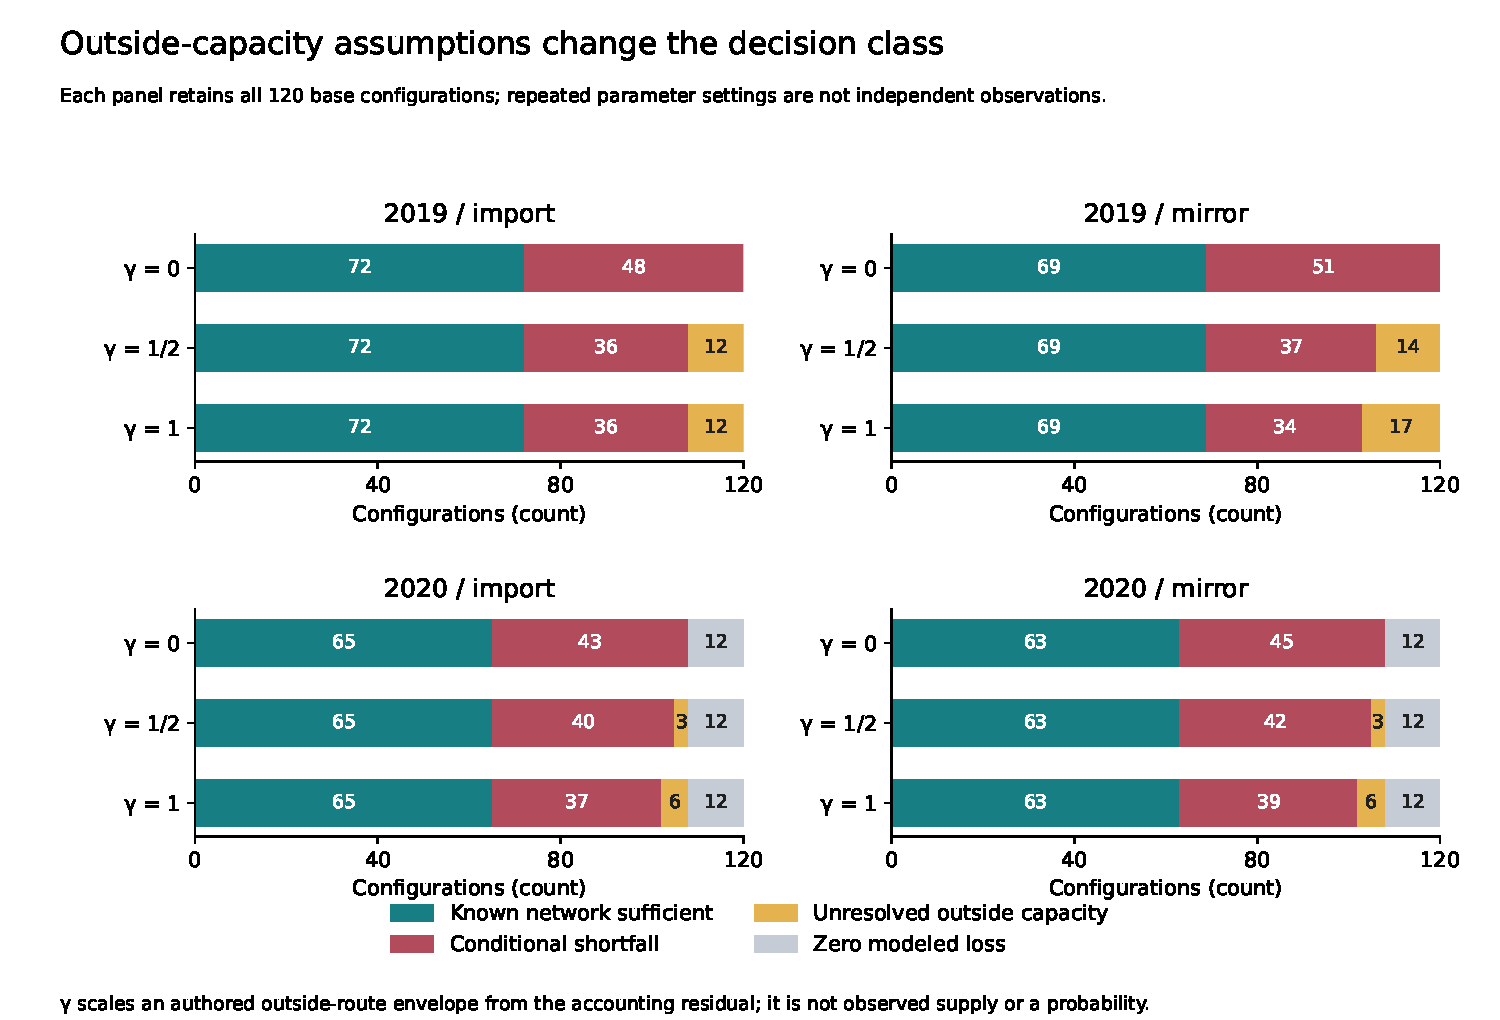
\includegraphics[width=.96\linewidth]{images/conditional_classes.pdf}\end{center}
The full-envelope U count is \BoundCG{} out of \BoundCH{} positive-loss configurations, counting both years and bases. The count describes this parameter grid, not the probability of a shortage or the fraction of independent real-world events. No outside supply is observed, and the envelope strengths are sensitivity assumptions rather than validated capacity estimates.

\newpage
\heading{Declared maximum-width illustration and shared-pool comparison}
The protocol requests the maximum interval width, retaining the first case in fixed year, source-basis, numeric parameter and origin order on ties. The selected example is \BoundCI{}, import basis, loss of \BoundCJ{}, $\alpha=\BoundCK{}$, $\beta=\BoundCL{}$. Its modeled demand is \BoundCM{} tonnes. At the full residual envelope, covered mass can range from \BoundCN{} to \BoundCO{} tonnes; unmet mass ranges from \BoundCP{} to \BoundCQ{} tonnes.

\begin{center}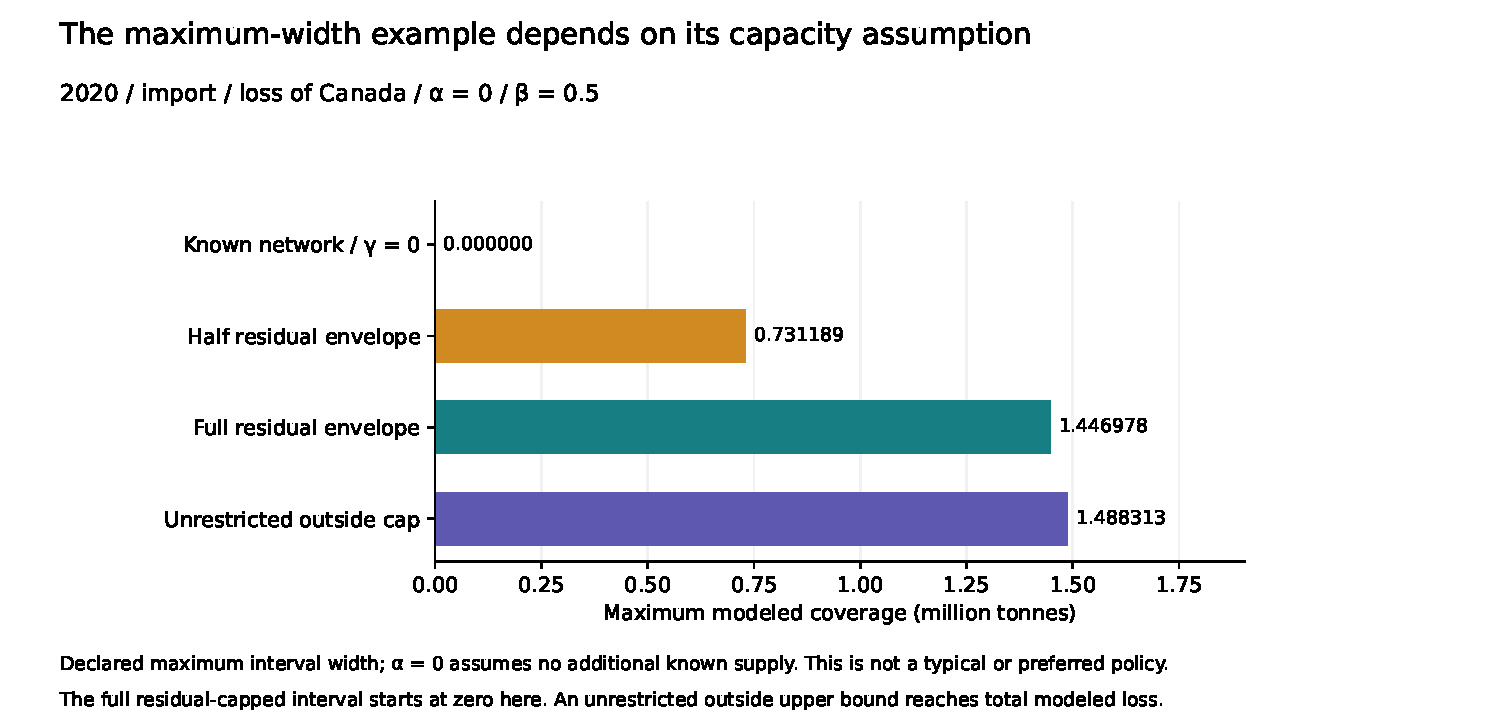
\includegraphics[width=\linewidth]{images/maximum_interval.pdf}\end{center}
The example has $\alpha=0$, so no additional known-origin supply is assumed. It is a declared maximum-width sanity/sensitivity case, not a typical loss, recommended policy or forecast. The half-envelope result in the chart comes from this same exact case; it need not equal half its full-envelope optimum because importer demands can bind. An unrestricted outside cap reaches total modeled demand by assumption.

\begin{center}\small\begin{tabular}{llrr}\toprule
Year & Known-only basis & Positive shared overclaims & Maximum gap (t)\\\midrule
2019 & import & \BoundCR{} & \BoundCS{}\\
2019 & mirror & \BoundCT{} & \BoundCU{}\\
2020 & import & \BoundCV{} & \BoundCW{}\\
2020 & mirror & \BoundCX{} & \BoundCY{}\\
\bottomrule\end{tabular}\end{center}
The shared-pool penalty is present in only four known-only mirror configurations in this grid. Source-basis sensitivity matters; mirror quantities are not truth and not independent corroboration. Every nonmaximum configuration, importer allocation, real/virtual supplier cap, slack and cut remains in the CSV accounts. No political priority is inferred from a tied maximum-flow allocation.

\newpage
\heading{Validation, execution order and practical use}
Native CSV/SQLite/70-digit Decimal reconciliation rechecks all four capture hashes and \BoundCZ{} requested source positions with 4,706 finite conditions, confirming the original failed gate. The new checker reconstructs source support, residuals, all capacities, complete flows/slacks and every cut without importing production scenario helpers. It passes \BoundDA{} conditions for 2019 and \BoundDB{} for 2020. All 56 authored fixture methods pass, including 20 new outside-boundary cases.

The original 39 source/code/test files remain byte unchanged. A development checker initially compared CSV integer strings directly with JSON integers; its failed receipt/code and unchanged development-result hashes are preserved privately. The checker representation was corrected before the actual 64-dependency development freeze at \texttt{f9d4de7a01a2818461df34c9767395d86d9d3654}. Later-year results use identical frozen methods, with no tuning or outcome-driven subset change. Both years' source values were already visible; this is not protected predictive validation.

Separate full-history CPython 3.10.11 and 3.12.14 replays reproduce all 14 primary files byte for byte, preserving all 23 source-directory files each. Independent summary/exercise checks pass \BoundDC{} conditions. The eight exercise requests return two qualified intervals, two abstentions and four rejections. The product requires a saved scenario and explicit outside envelope; it rejects shipment guarantees, shortage probabilities, political priority and arbitrary caller data.

Run \texttt{python src/bounds\_replay.py --out ../bounds-replay} with the pinned requirements and a new output directory. Before a real delivery promise, obtain supplier-specific available volumes, compatible grain grades, freight/contract constraints and independently dated routing evidence. A mathematically feasible allocation is not an available commercial shipment.

\heading{Limits, sources and publication boundary}
This small country-level grain network omits domestic production, nutrition, inventories, prices, harvest timing and commodity-grade compatibility. Compiled import/mirror sources, imputed values, reporting territories and revision histories can differ. Scenario counts reuse annual inputs and shared origins. No p-value, probability, calibrated confidence interval, current food-risk assessment, causal benefit, deployment or saving is established. Residual-scaled caps are explicit hypotheses, not inferred physical bounds. The original coverage-gated study remains unexecuted.

[1] FAO/FAOSTAT, \href{https://www.fao.org/faostat/en/#data/TM/metadata}{Detailed trade matrix} and \href{https://www.fao.org/faostat/en/#data/TCL/metadata}{Crops and livestock products trade}. Wheat item definitions and source-specific metadata/flags are retained in the source plan and receipts. Authors convert units, filter support and construct new scenarios; publishers are not responsible for these changes and do not endorse them.

[2] \href{https://www.fao.org/contact-us/terms/db-terms-of-use/en/}{FAO database terms}, with \href{https://uncomtrade.org/docs/re-dissemination-of-data/}{UN redistribution} and \href{https://ec.europa.eu/eurostat/help/copyright-notice}{Eurostat copyright} restrictions. Minimal attributed facts only; no bulk/resale service or unrestricted commercial source license. Native exports, contacts, credentials and expressive source material stay private. MIT covers original code.

[3] MIT OpenCourseWare, \href{https://ocw.mit.edu/courses/18-200-principles-of-discrete-applied-mathematics-spring-2024/resources/18200-lecture-15-version-2_mp4/}{Max-Flow Min-Cut Theorem}, established method context. This finite implementation claims no new algorithm or exhaustive scientific priority. Independent-program manuscript, not peer reviewed or formally submitted. Azure and other formal-publication projects remain private.
\end{document}
